%%%%%%%%%%%%%%%%%%%%%%%%%%%%%%%%%%%%%%%%%%%%%%%%%%%%%%%%%%%%%%%%%%%%%%%%%%%%%%%
%
% Evaluation
% 
%%%%%%%%%%%%%%%%%%%%%%%%%%%%%%%%%%%%%%%%%%%%%%%%%%%%%%%%%%%%%%%%%%%%%%%%%%%%%%%


\chapter{Results and Discussion}
\label{sec:results}

The work of \citet{zhou1999vortex} is replicated in this thesis study. The characteristics of an elastically mounted circular cylinder suspended in a fluid domain is studied. The cylinder is free to oscillate in x and y direction, so two-Dimensional study is conducted. According to \citet{williamson1996vortex}, the upper limit of Reynolds number (Re) where the vortex shedding from a circular cylinder is still two-dimensional and the wake is laminar can reach 200. In the current study a laminar flow is considered with $Re=200$ which is the same as that of \citet{zhou1999vortex}. The inlet flow velocity is set to $U_\infty = 1 \frac{m}{s}$, the fluid density is considered as $\rho = 1 \frac{kg}{m^3}$ and the flow viscosity is calculated to be $\mu=\frac{1}{200} Pa s$. These factors are tabulated as shown in \ref{table:4.1}. 

\begin{table}[H]
 \centering
	\begin{tabular}{|c|c|}
		\hline 
		Parameter & Value\tabularnewline
		\hline 
		Re & 200\tabularnewline
		\hline 
		U {[}m/s{]} & 1\tabularnewline
		\hline 
		D {[}m{]} & 1\tabularnewline
		\hline 
		$\mu$ {[}Pa s{]} & 1/200\tabularnewline
		\hline 
		$\rho$ {[}$\frac{kg}{m^{3}}${]} & 	1\tabularnewline
		\hline 
	\end{tabular}
\caption{Laminar flow properties and the diameter of the cylinder considered}
\label{table:4.1}
\end{table}

\section{Computational Grid}

A 2-D \textit{O-Grid} mesh is generated around the cylinder. The first cell is placed at a distance of $0.0025*D$ from the cylinder wall. The growth rate is set to $1.05$, a total of $240x200 (r x \theta)$ control volumes are generated for the domain. The distance from the cylinder to the outer boundary is considered to be $15*D$. Two blocks are generated which is further split into 4 blocks each, along the radial axis for grid parallelization. Since this is a two-dimensional analysis, span-wise grid is not refined or resolved. A time step size of 0.001 s is considered for the current study. 

The selected time step leads to a maximum Courant number of around 0.4. The maximum Courant number $(C_{max})$ is a dimensionless number which is obtained
by evaluating the Courant-Friedrichs-Lewy condition or CFL condition which can be written as   
\begin{equation}
C = \frac{u \Delta t}{\Delta x} \leq C_max
\label{eqn:4.1} 
\end{equation}

where C is the dimensionless Courant number in every time-step.

The generated grid, inlet and outlet boundary patches considered are highlighted in the figure \ref{fig:4.1}.
\begin{figure}[h]
%\centering
	\begin{minipage}[t]{4cm}
		\fbox{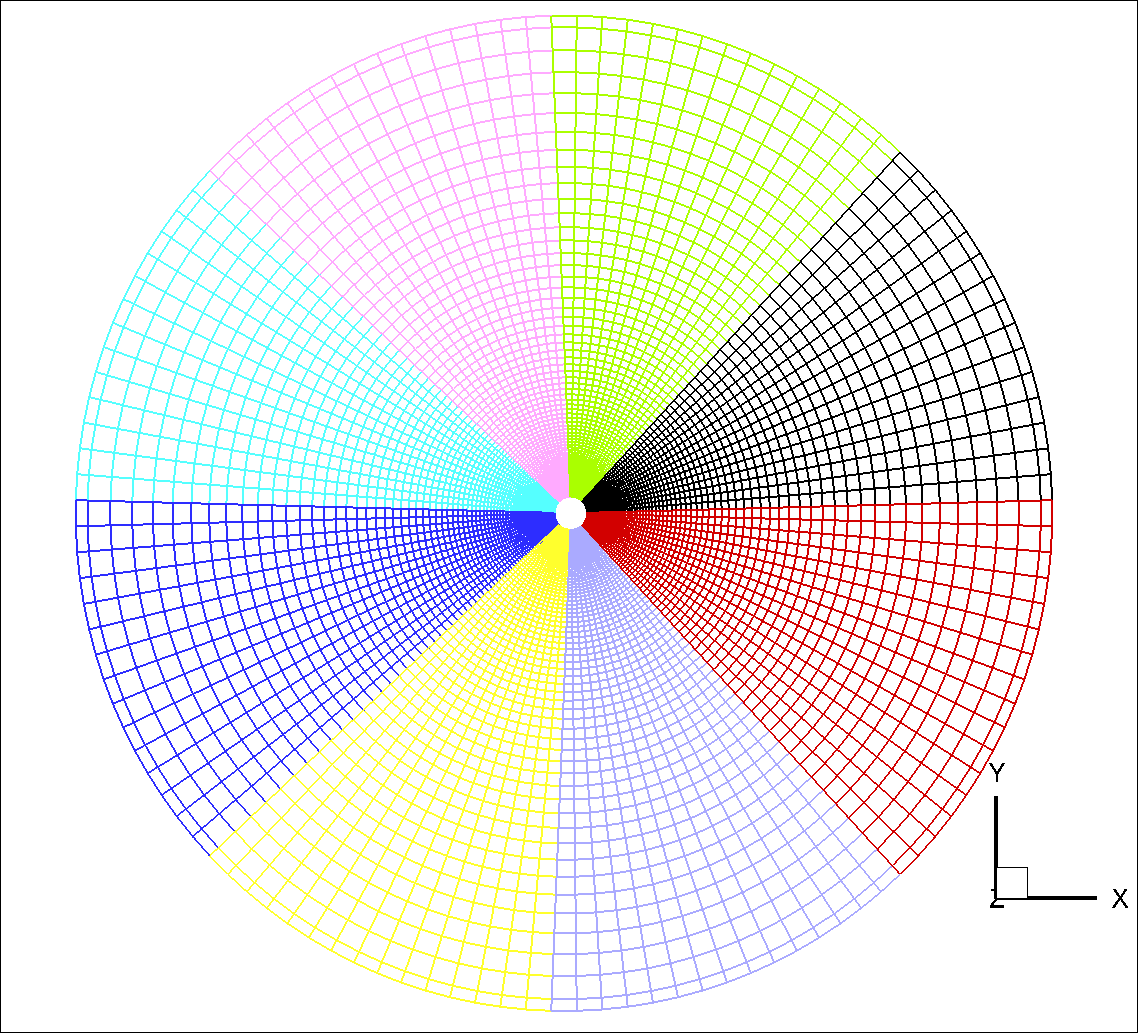
\includegraphics[height=2.65in]{grid}}
%		\caption{Grids colored by blocks of parallelization}
	\end{minipage}
	\hspace{4cm}
	\begin{minipage}[t]{4cm}
%		\centering
		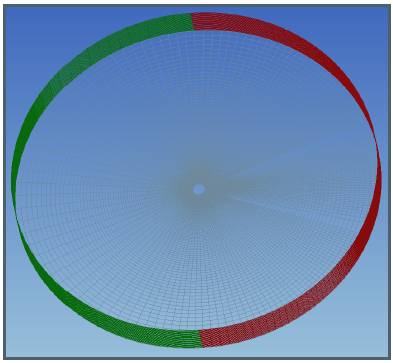
\includegraphics[height=2.65in]{grid_inout}
%		\caption{Grids colored by blocks of parallelization}
	\end{minipage}
\caption{Left: Grids colored by blocks of parallelization; Right: Grid highlighted with inlet (Green) and outlet(Red) patches}
\label{fig:4.1}
\end{figure}

This same mesh has been used for all the simulations in the current study.

\section{Results of flow analysis}
Initially a flow analysis for a flow around a fixed cylinder is conducted. In FASTEST-3D, convective boundary conditions are implemented for outlet boundaries in order to overcome the short-comings of zero-gradient outlet. The convective boundary conditions are implemented by solving explicitly a convective transport equation. The convective transport equation can be written in the form
\[ \frac {\partial U_i}{\partial t} + \frac{\partial U^c_j
  U_i}{\partial x_j} = 0 ~; 
\]
which equals to 
\[ \frac {\partial U_i}{\partial t} + U^c \frac{\partial U_i}{\partial
  x} + V^c \frac{\partial U_i}{\partial y} + W^c \frac{\partial
  U_i}{\partial z}   = 0 ~,
\]

where $ U^c_j = ( U^c V^c W^c )^T $ is the velocity vector of the
convection.\\

The boundary conditions used for the simulation is tabulated in \ref{table:4.2}. The simulation is run for a total of 200,000 time-steps, i.e. for a physical time of 200s. 

\begin{table} [H]
\centering
	\begin{tabular}{|c|c|}
	\hline 
	Boundary  & Boundary condition \tabularnewline
	\hline 
	\multirow{2}{*}{Inlet} & Velocity Inlet \tabularnewline
	\cline{2-2} 
	 & $U_{x}$ = 1 m/s \tabularnewline
	\hline 
	\multirow{2}{*}{Outlet} & Convective boundary \tabularnewline
	\cline{2-2} 
	 & $U^{c}$ = 1\tabularnewline
	\hline 
	\end{tabular}
\caption{Boundary conditions considered for the simulation}
\label{table:4.2}
\end{table}

In the figure \ref{fig:4.2} the instantaneous velocity field behind the cylinder is presented. In can be observed that right behind the cylinder the vortices has maximum energy and as these vortices travel further down-stream the energy dissipates. By the time the vortices reaches the limit of the domain all the energy has been dissipated and vortices vanishes. The alternating vortex shedding can also be
observed from the instantaneous pressure contour in figure \ref{fig:4.3}. The vortex pattern in the wake composes of negative and positive staggered vortices, that is commonly referred to as \textit{Karman vortex street}. The shed vortices from the cylinder follows almost identical path downstream.  

%\begin{figure}[h]
%%\centering
%	\begin{minipage}[t]{4cm}
%		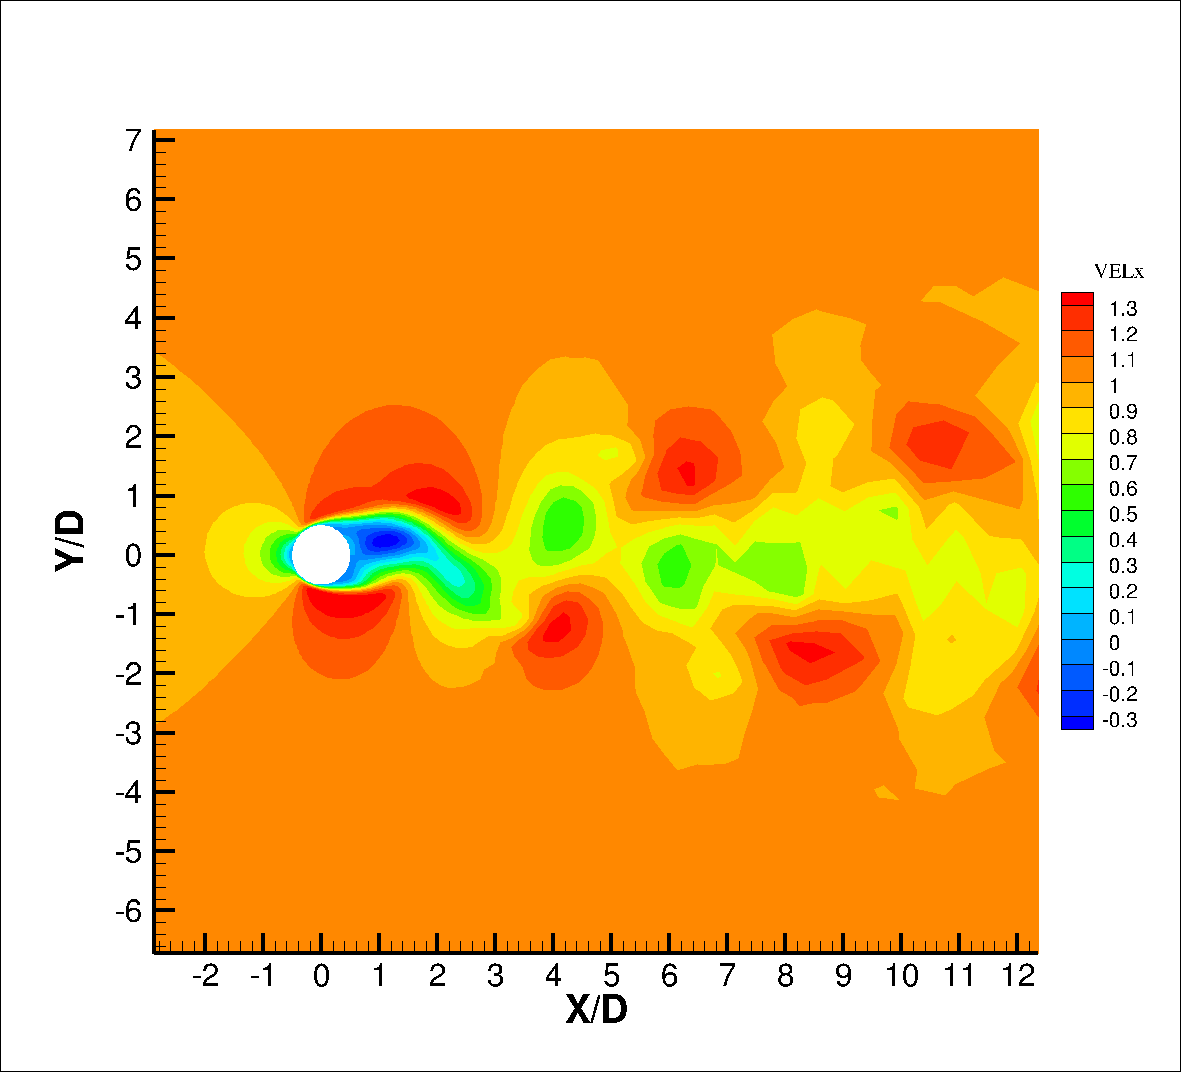
\includegraphics[height=2.6in]{Vx_181s}
%		\caption{t=181s}
%	\end{minipage}
%	\hspace{4cm}
%	\begin{minipage}[t]{4cm}
%%		\centering
%		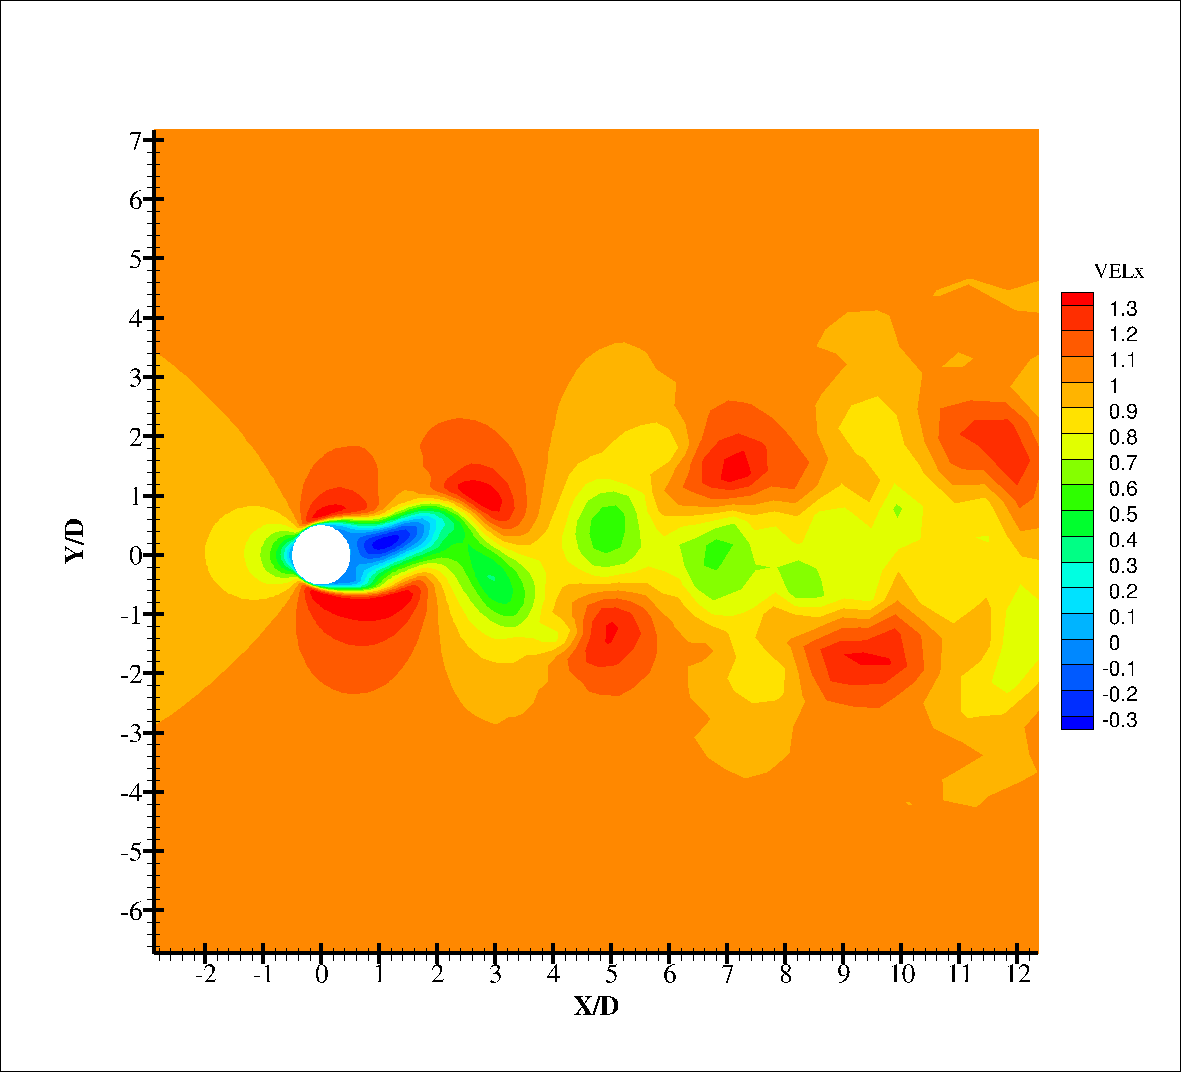
\includegraphics[height=2.6in]{Vx_182s}
%		\caption{t=182s}
%	\end{minipage}
%	
%	\begin{minipage}[t]{4cm}
%		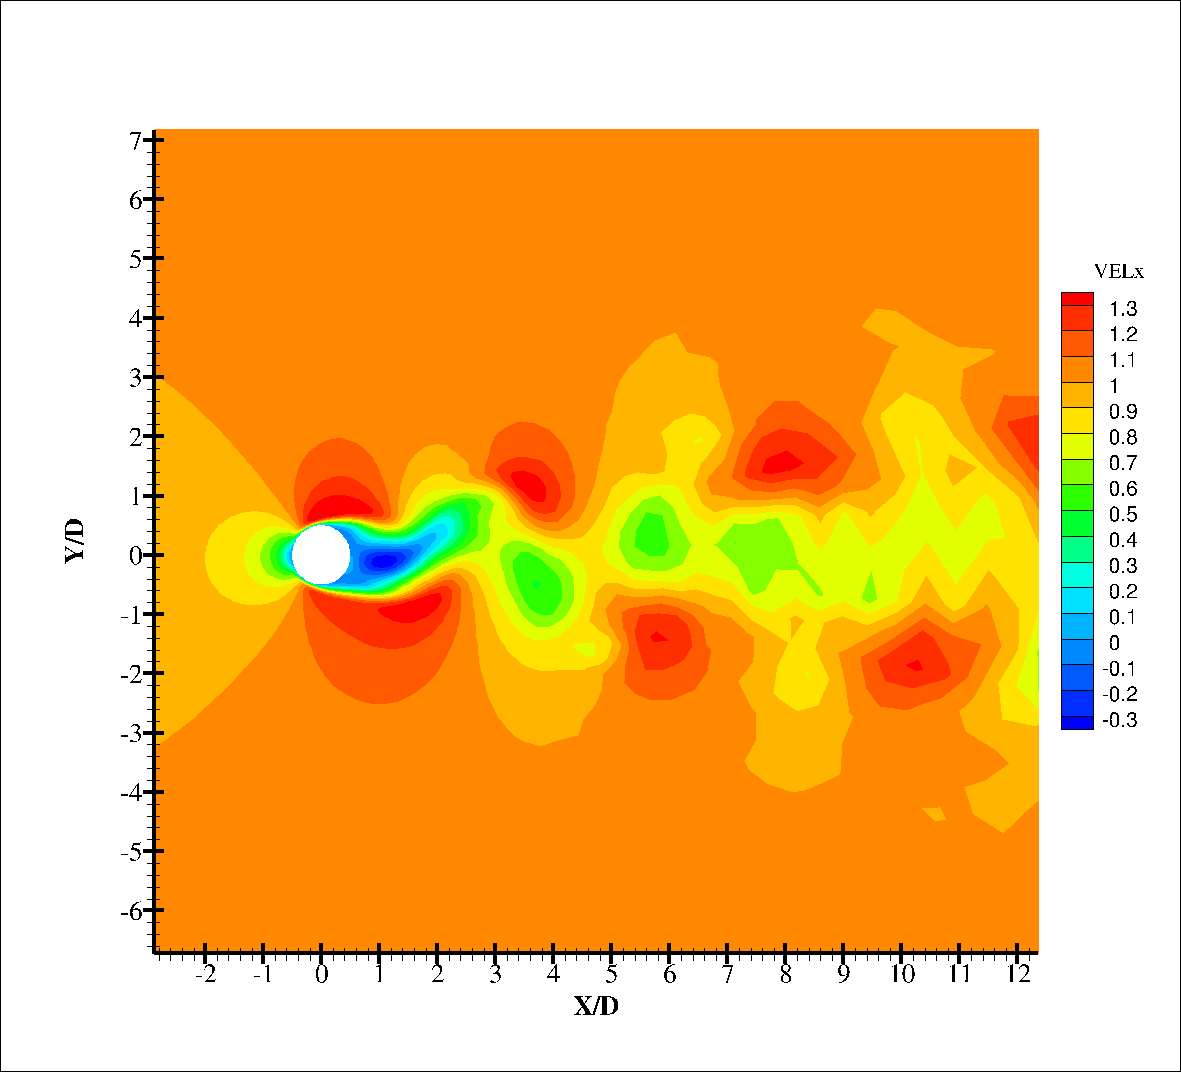
\includegraphics[height=2.6in]{Vx_183s}
%		\caption{t=183s}
%	\end{minipage}
%	\hspace{4cm}
%	\begin{minipage}[t]{4cm}
%%		\centering
%		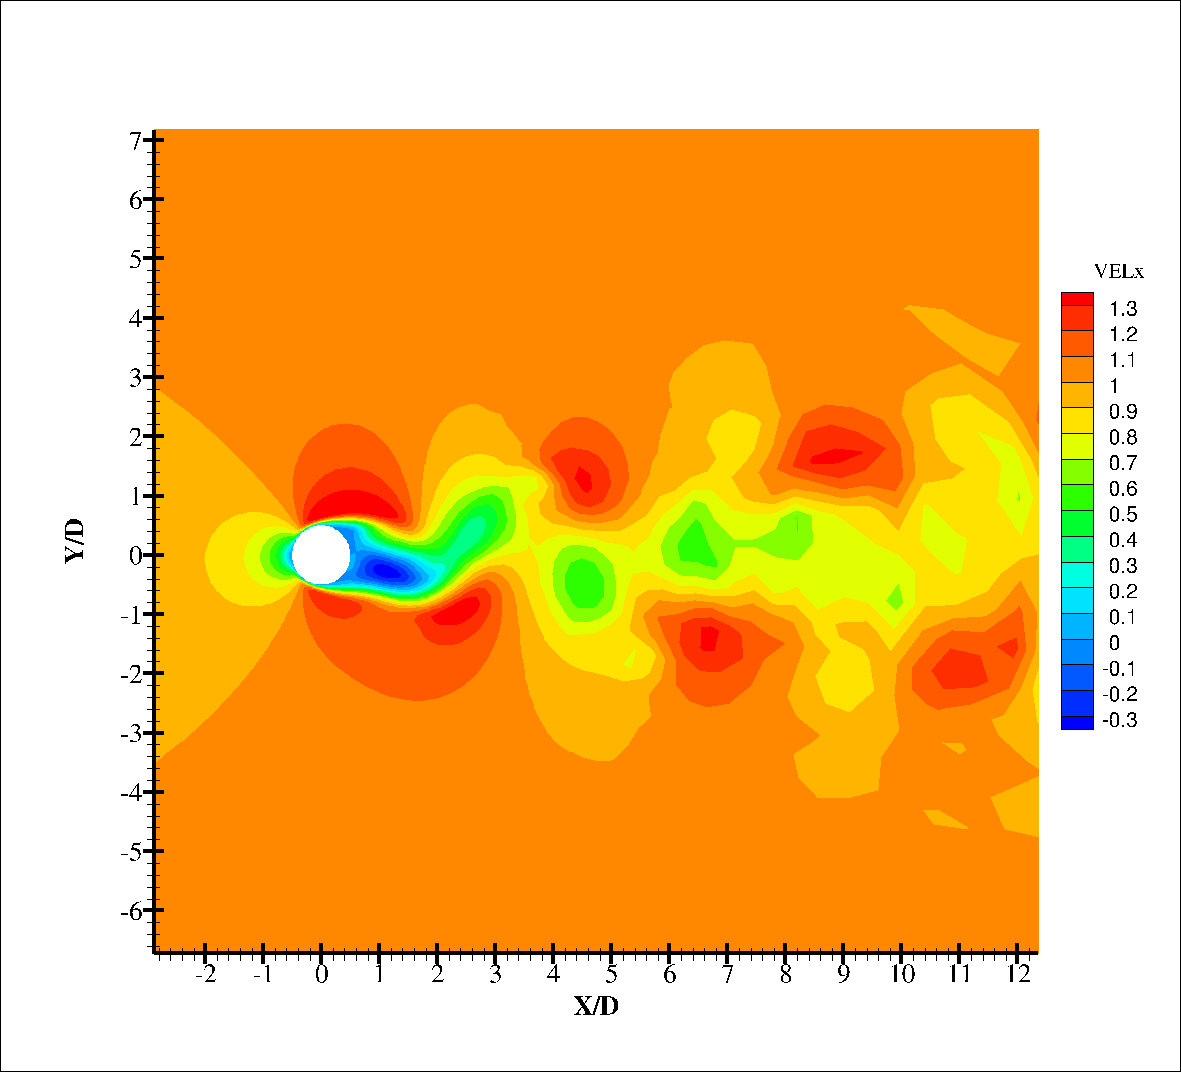
\includegraphics[height=2.6in]{Vx_184s}
%		\caption{t=184s}
%	\end{minipage}
%	
%	\begin{minipage}[t]{4cm}
%		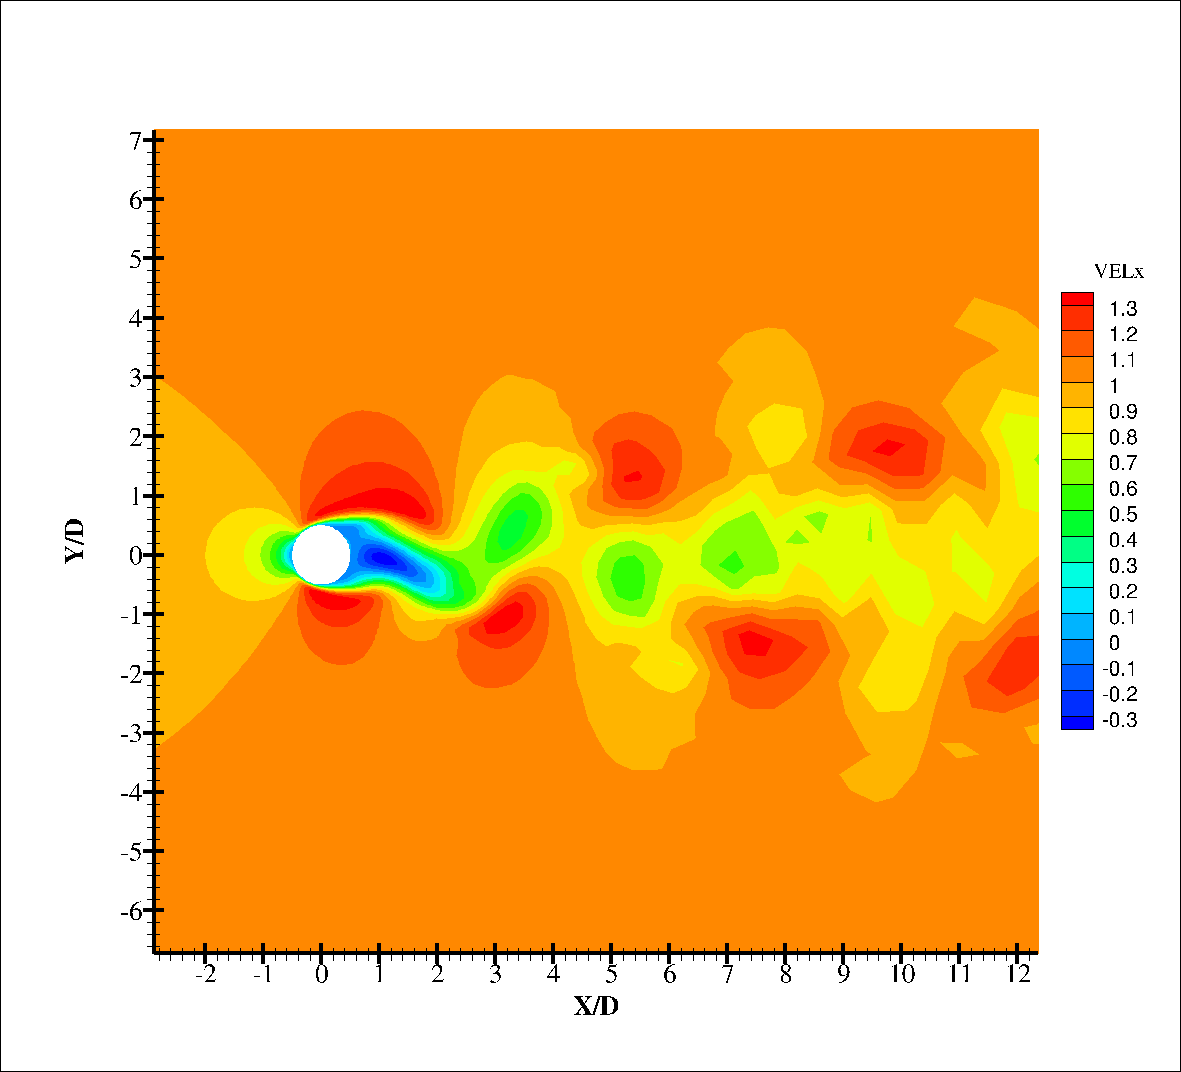
\includegraphics[height=2.6in]{Vx_185s}
%		\caption{t=185s}
%	\end{minipage}
%	\hspace{4cm}
%	\begin{minipage}[t]{4cm}
%%		\centering
%		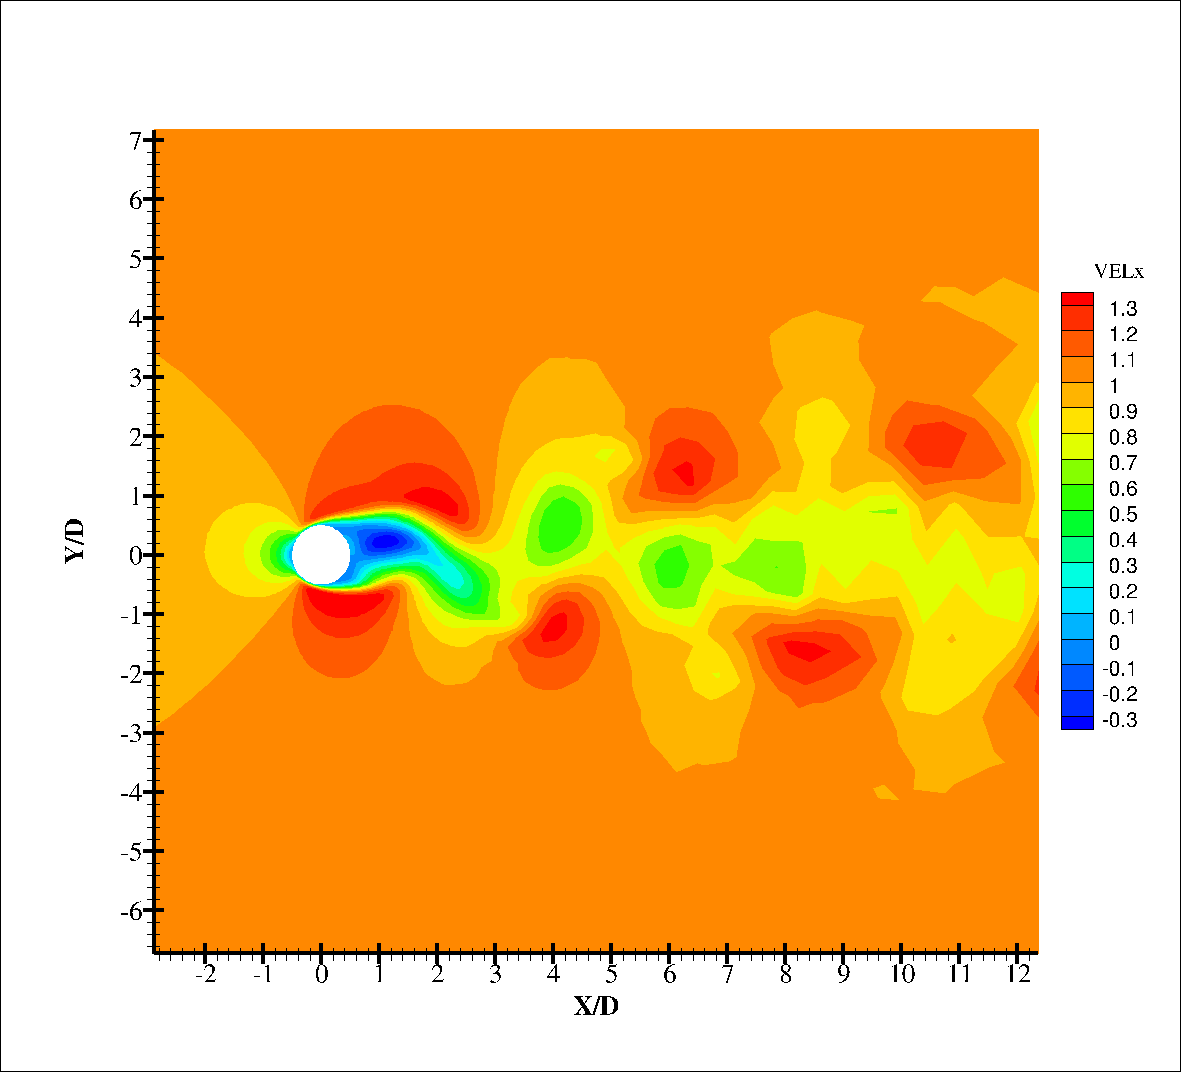
\includegraphics[height=2.6in]{Vx_186s}
%		\capt[ion{t=186s}
%	\end{minipage}
%\caption{Instantaneous velocity contour}
%\label{fig:4.2}
%\end{figure}

\begin{figure}[H]
\centering
	\begin{subfigure}[t]{7cm}
		\fbox{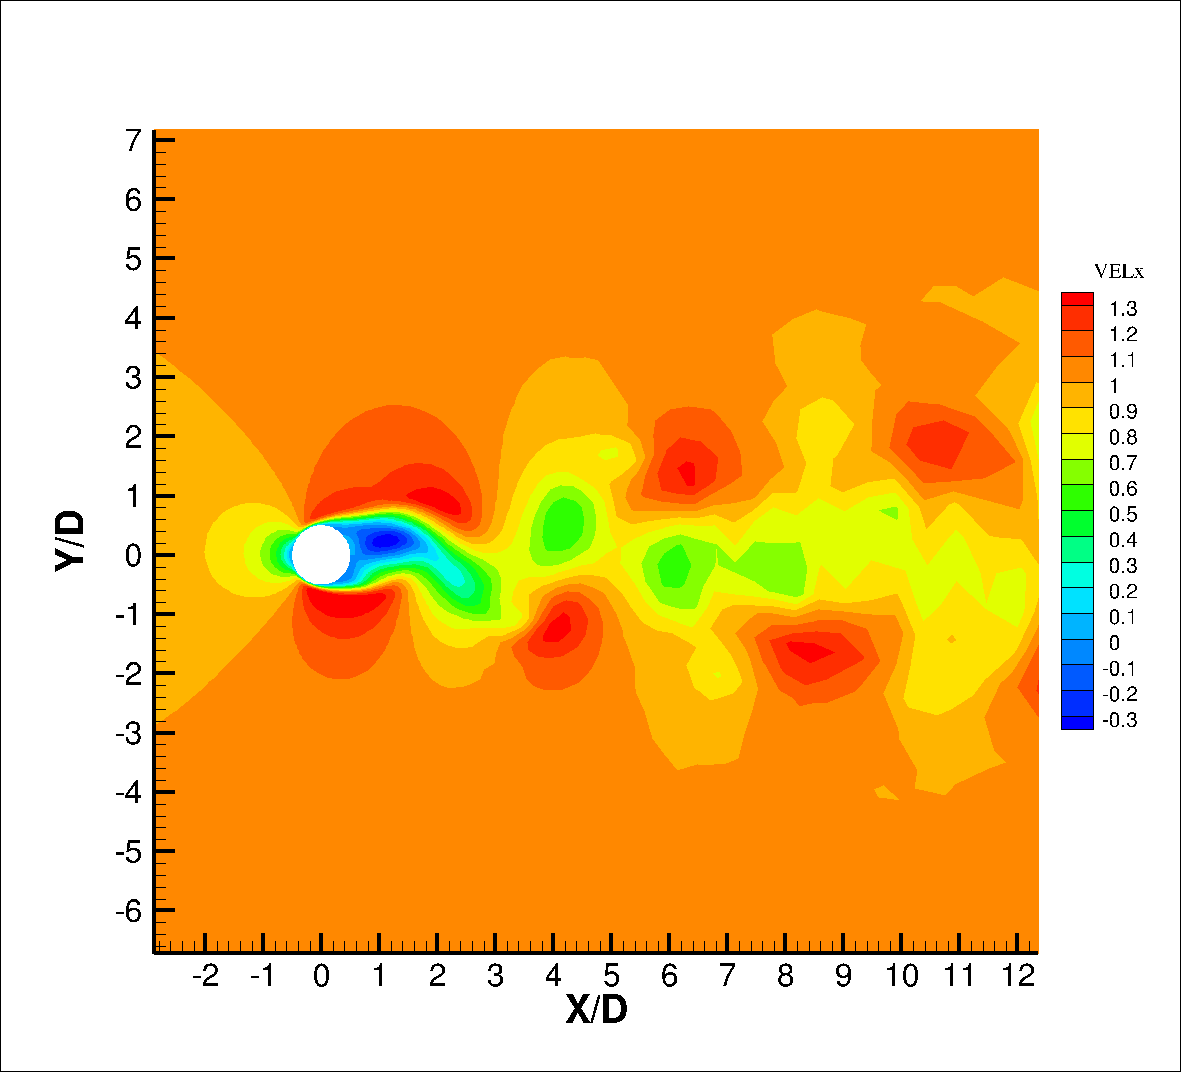
\includegraphics[width=6.5cm]{Vx_181s}}
		\caption{t=181s}
	\end{subfigure}
%	\hspace{4cm}
	\begin{subfigure}[t]{7cm}
%		\centering
		\fbox{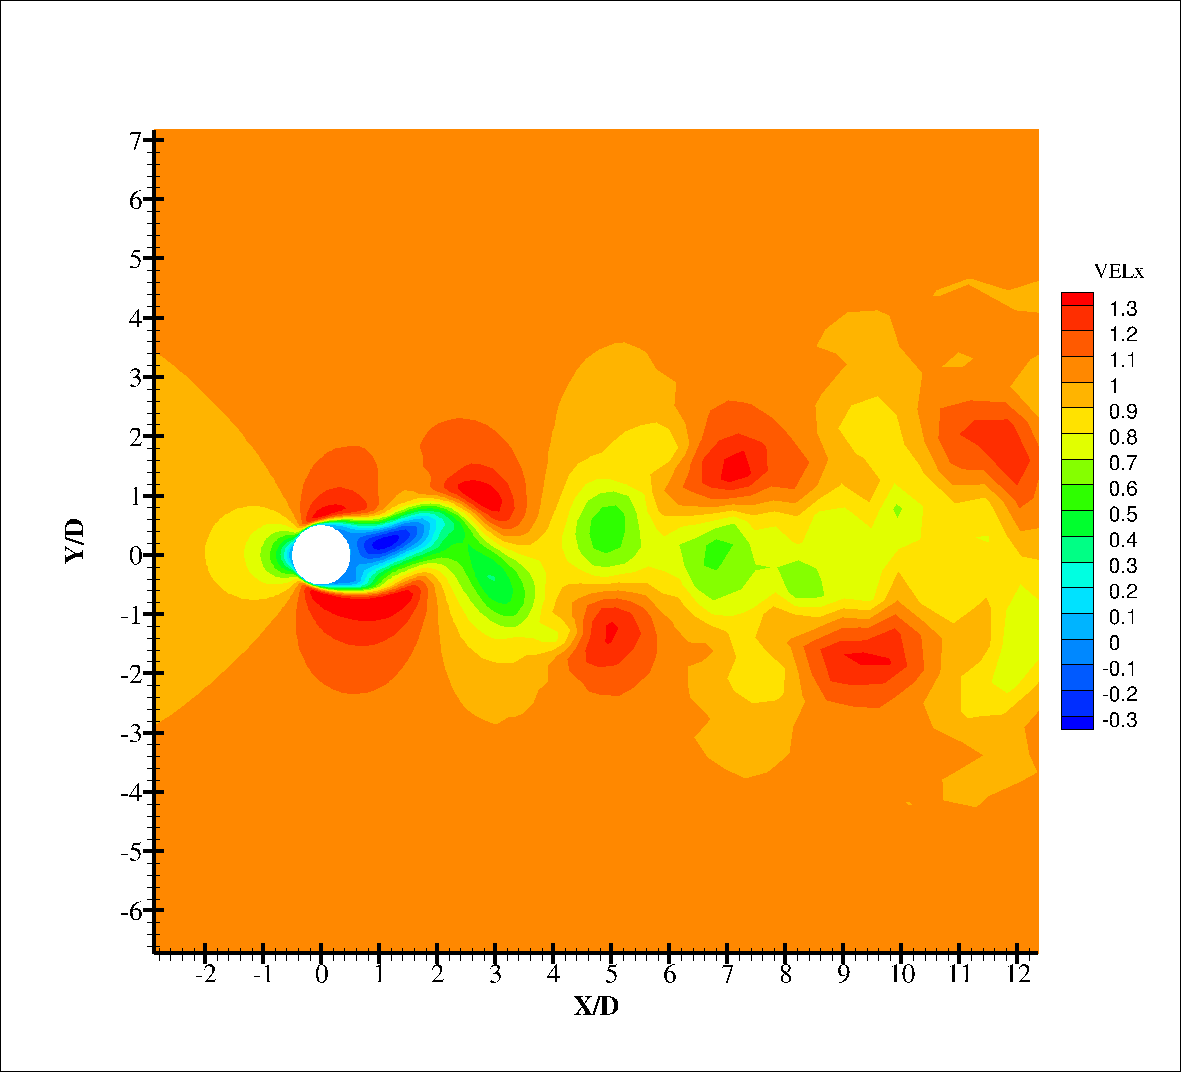
\includegraphics[width=6.5cm]{Vx_182s}}
		\caption{t=182s}
	\end{subfigure}
	
	\begin{subfigure}[t]{7cm}
		\fbox{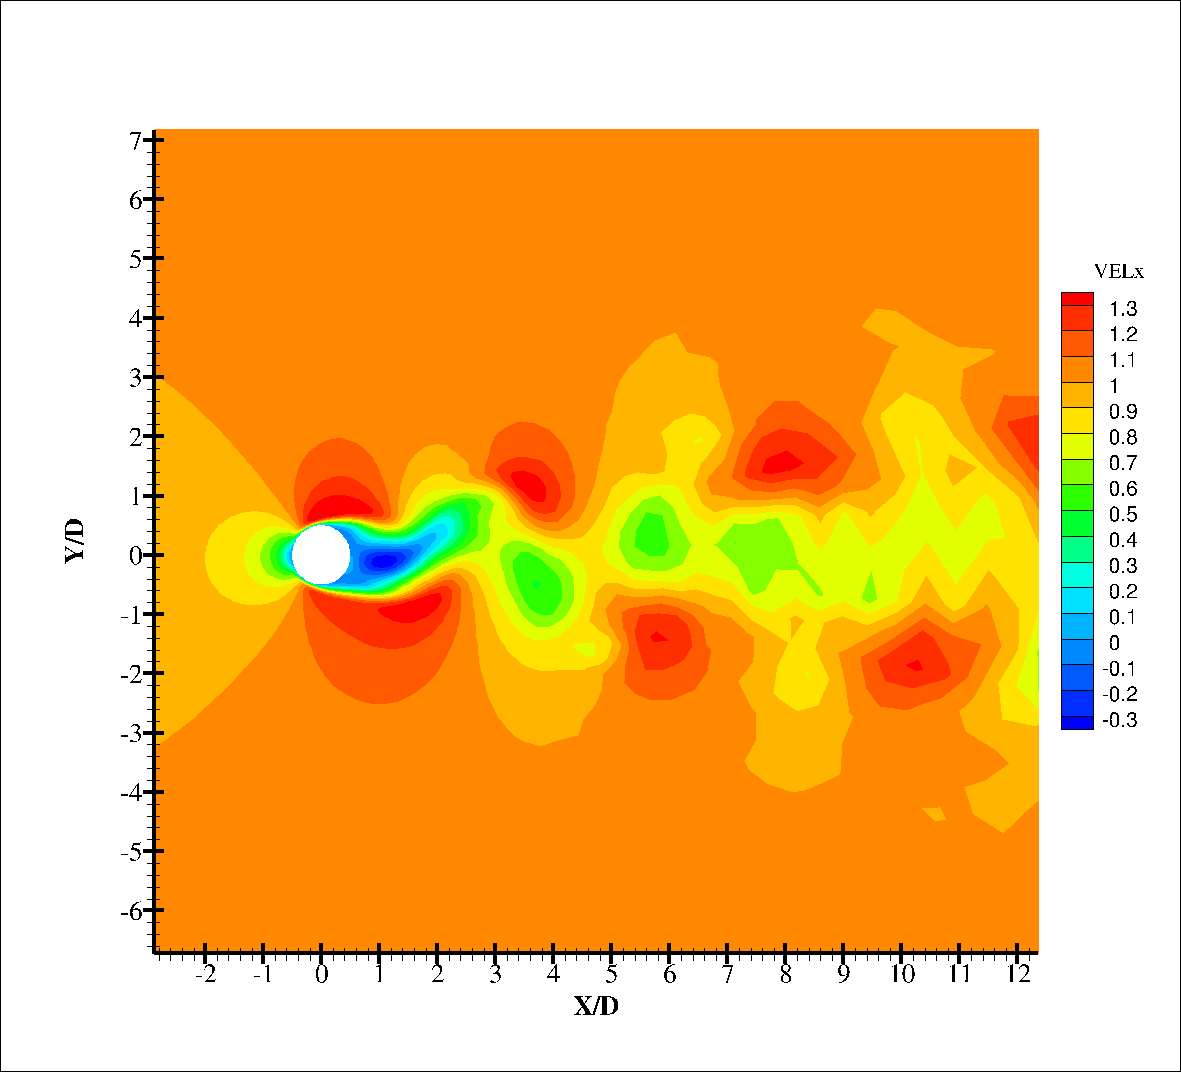
\includegraphics[width=6.5cm]{Vx_183s}}
		\caption{t=183s}
	\end{subfigure}
%	\hspace{4cm}
	\begin{subfigure}[t]{7cm}
%		\centering
		\fbox{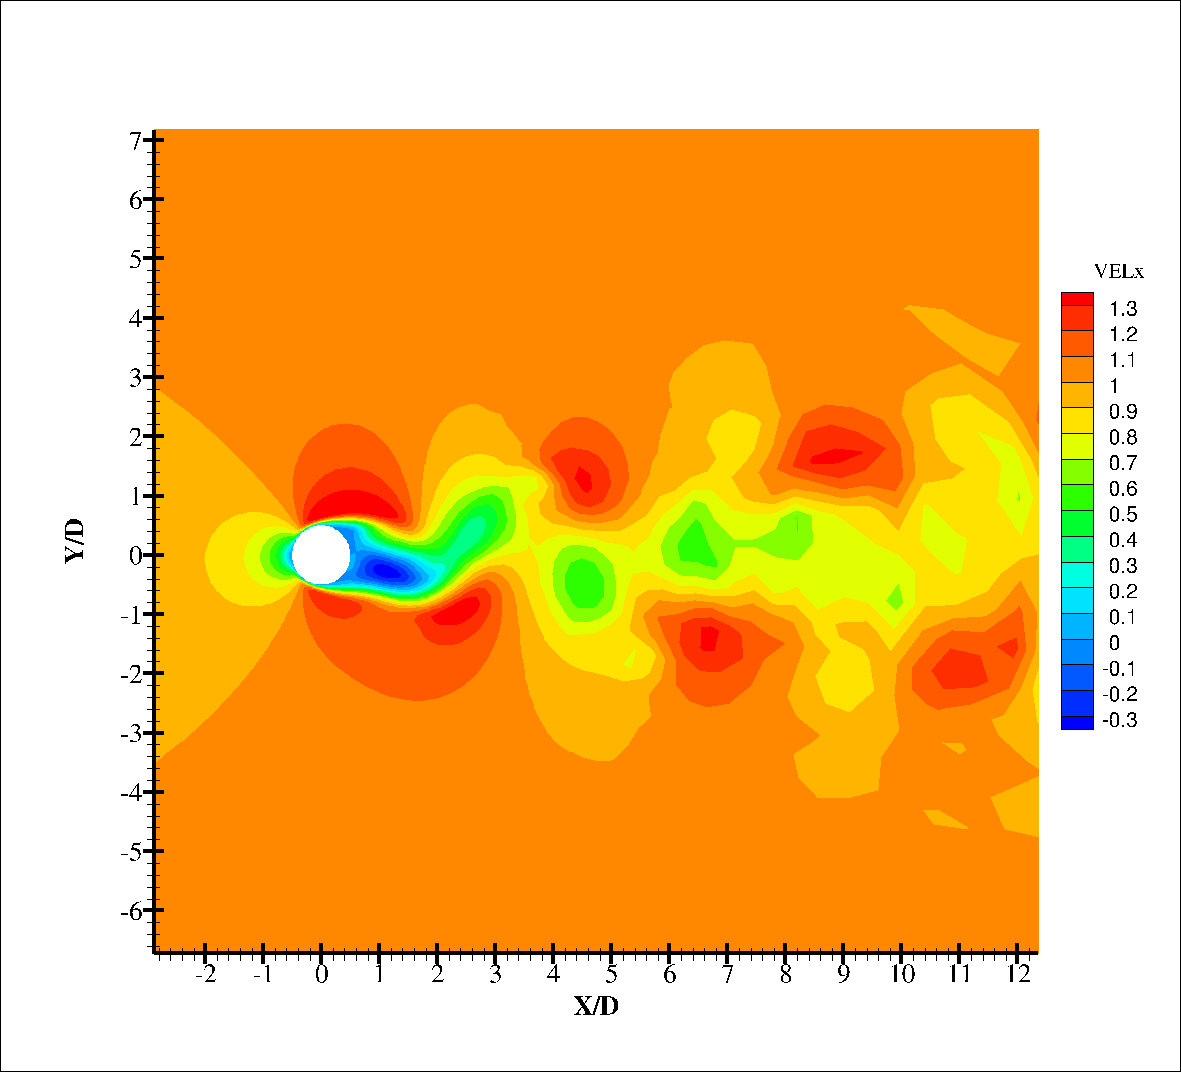
\includegraphics[width=6.5cm]{Vx_184s}}
		\caption{t=184s}
	\end{subfigure}
	
	\begin{subfigure}[t]{7cm}
		\fbox{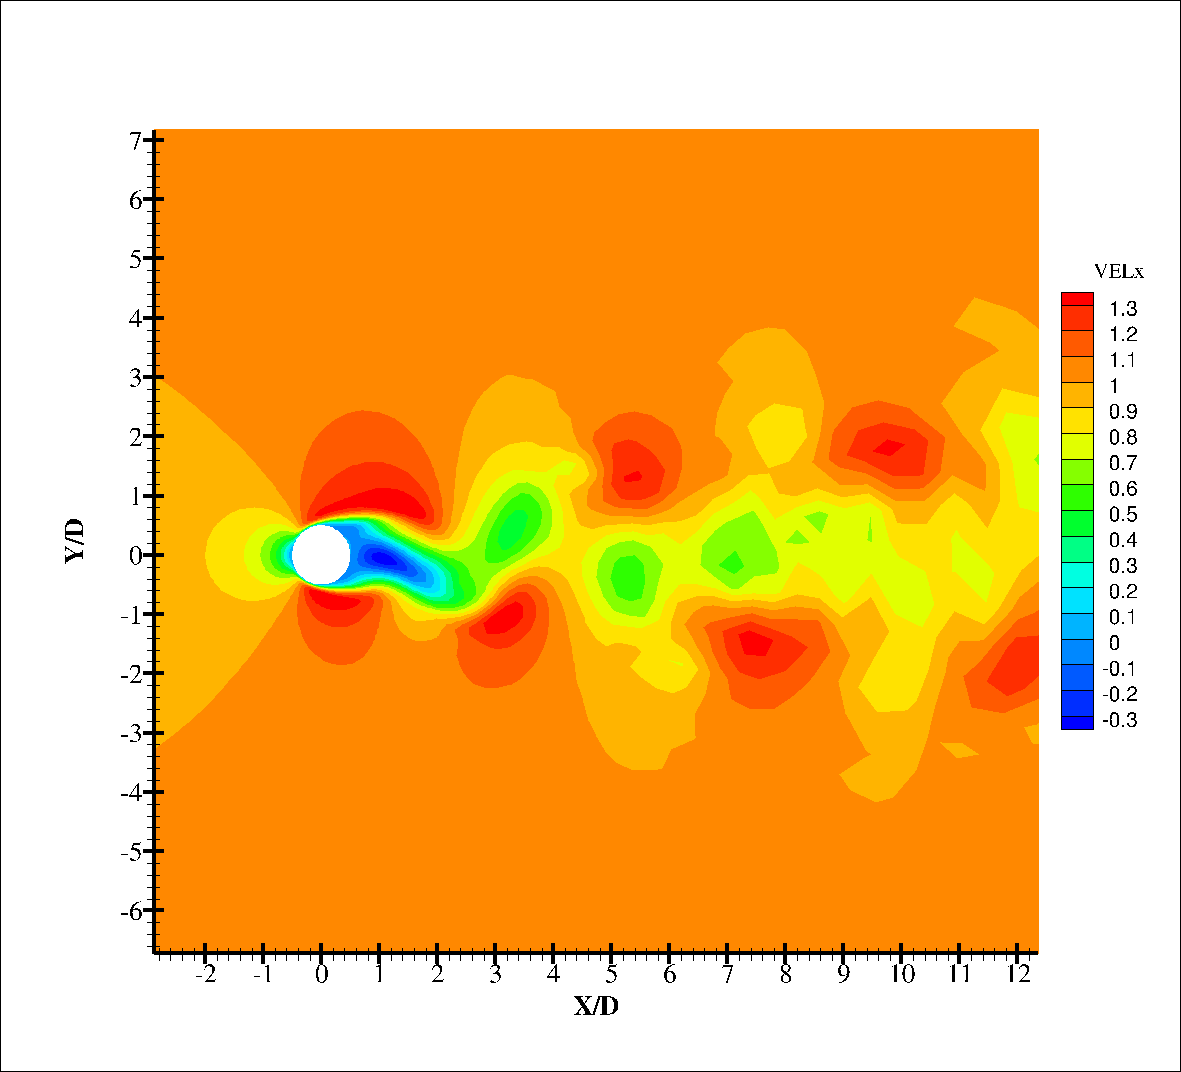
\includegraphics[width=6.5cm]{Vx_185s}}
		\caption{t=185s}
	\end{subfigure}
%	\hspace{4cm}
	\begin{subfigure}[t]{7cm}
%		\centering
		\fbox{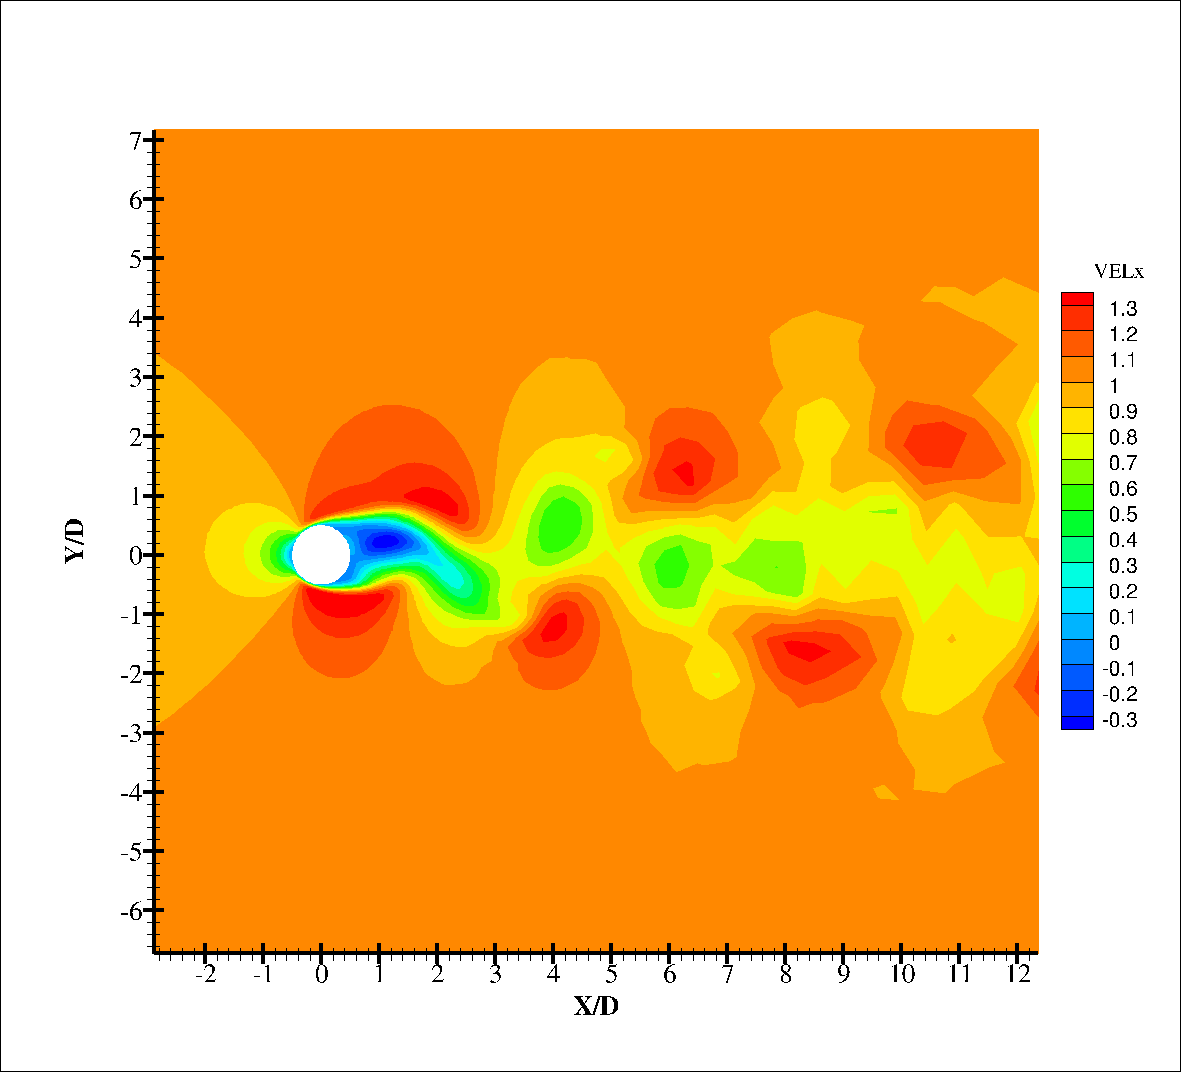
\includegraphics[width=6.5cm]{Vx_186s}}
		\caption{t=186s}
	\end{subfigure}
\caption{Instantaneous velocity contour}
\label{fig:4.2}
\end{figure}

\begin{figure}[H]
\centering
	\begin{subfigure}[t]{7cm}
		\fbox{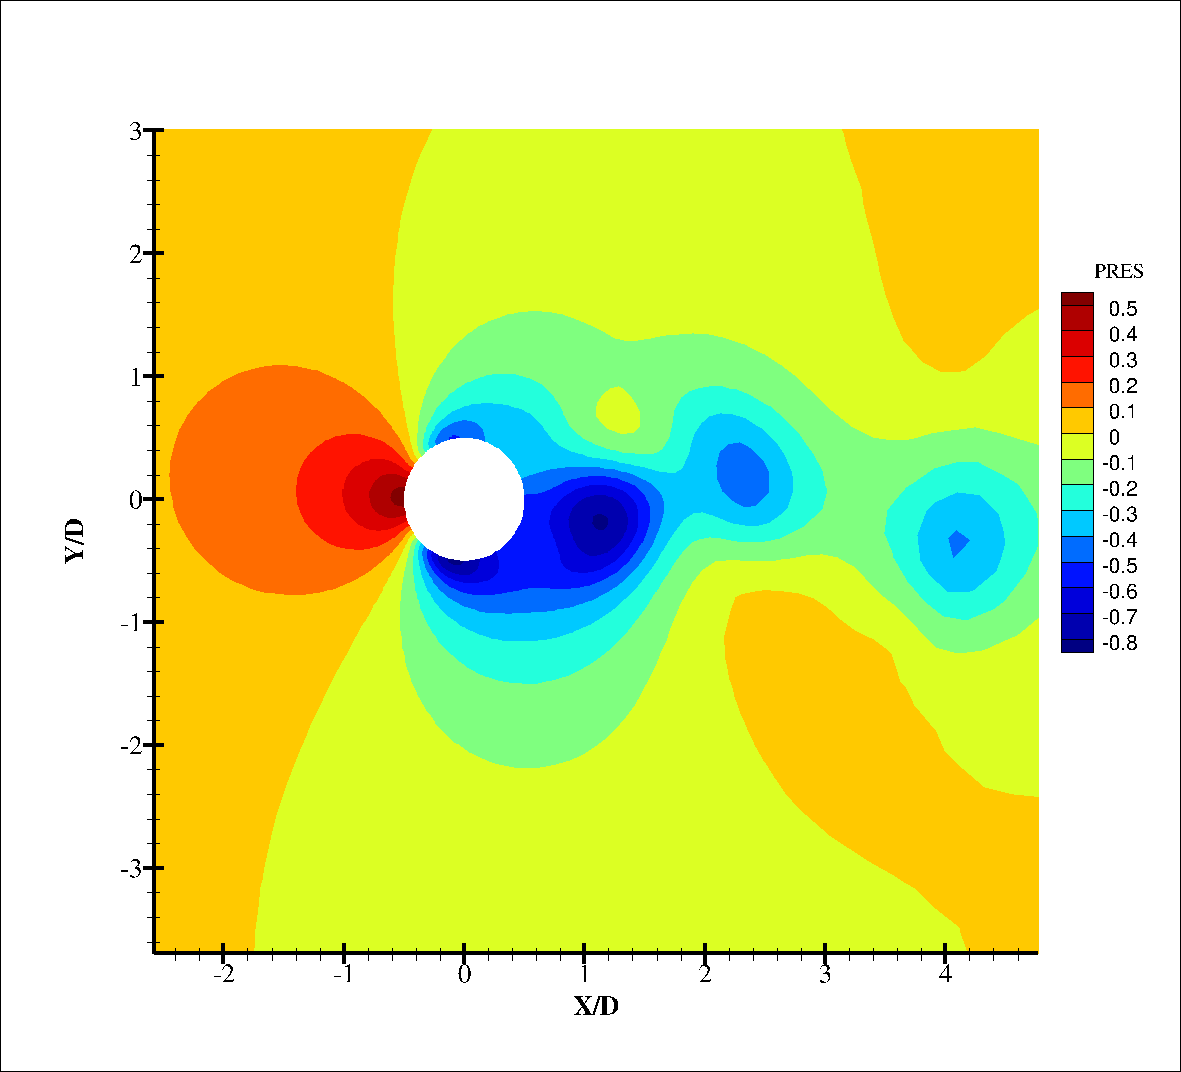
\includegraphics[width=6.5cm]{Pr_cyl_181s}}
		\caption{t=181s}
	\end{subfigure}
%	\hspace{4cm}
	\begin{subfigure}[t]{7cm}
%		\centering
		\fbox{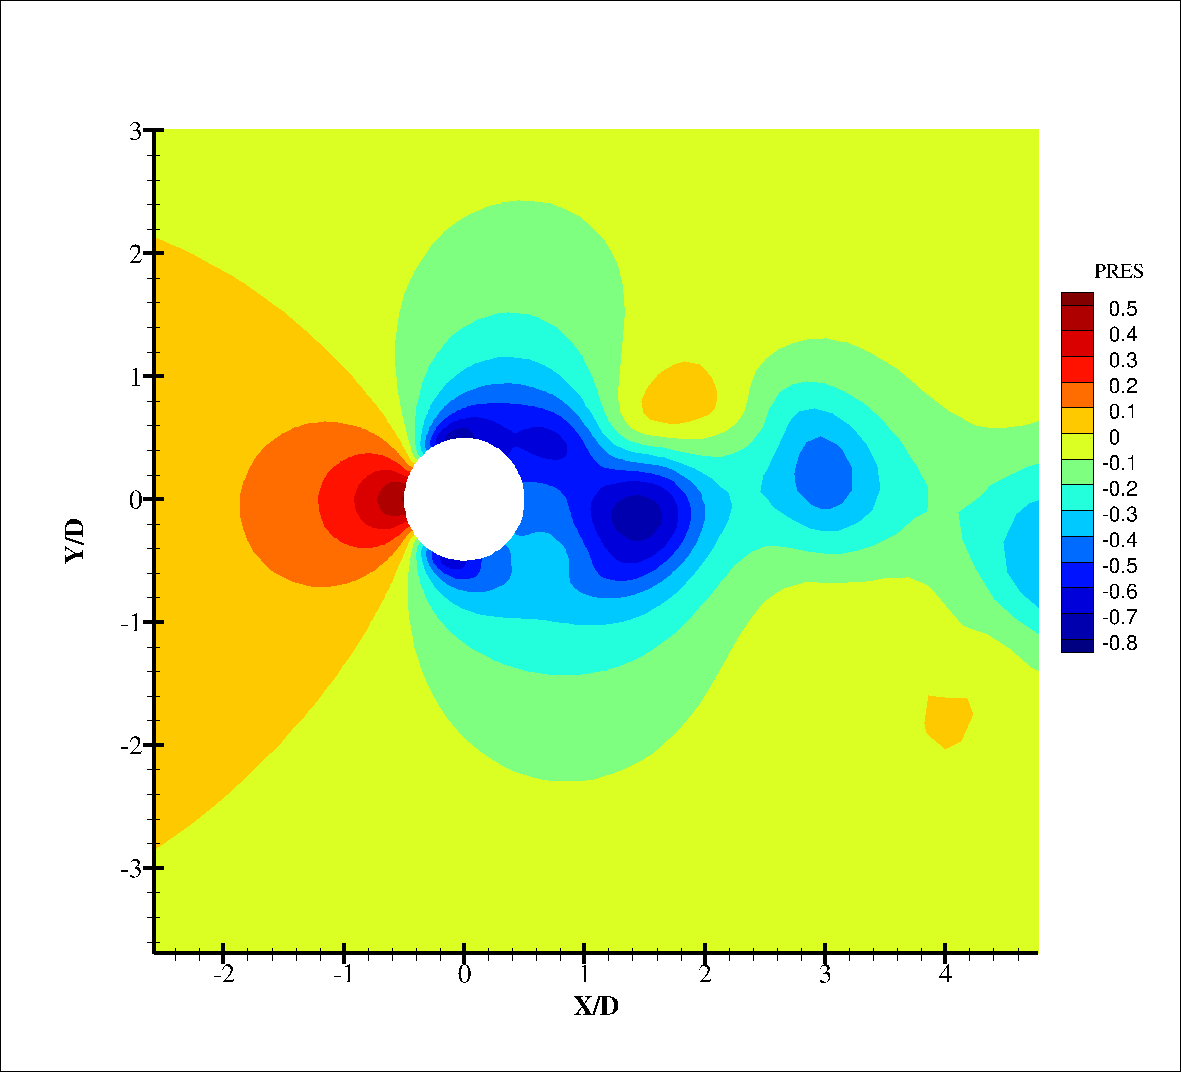
\includegraphics[width=6.5cm]{Pr_cyl_182s}}
		\caption{t=182s}
	\end{subfigure}
	
	\begin{subfigure}[t]{7cm}
		\fbox{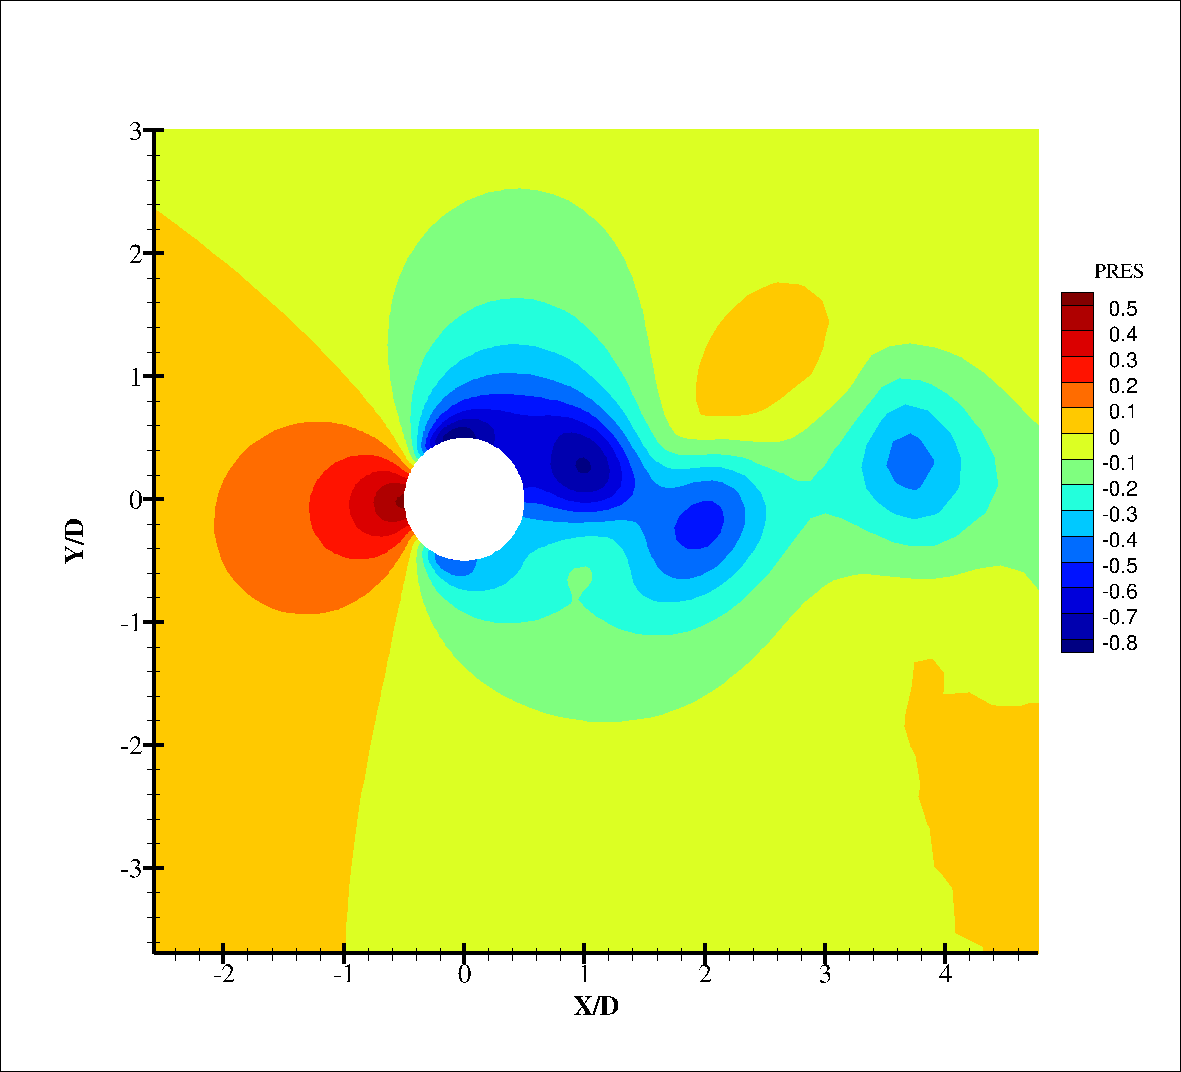
\includegraphics[width=6.5cm]{Pr_cyl_183s}}
		\caption{t=183s}
	\end{subfigure}
%	\hspace{4cm}
	\begin{subfigure}[t]{7cm}
%		\centering
		\fbox{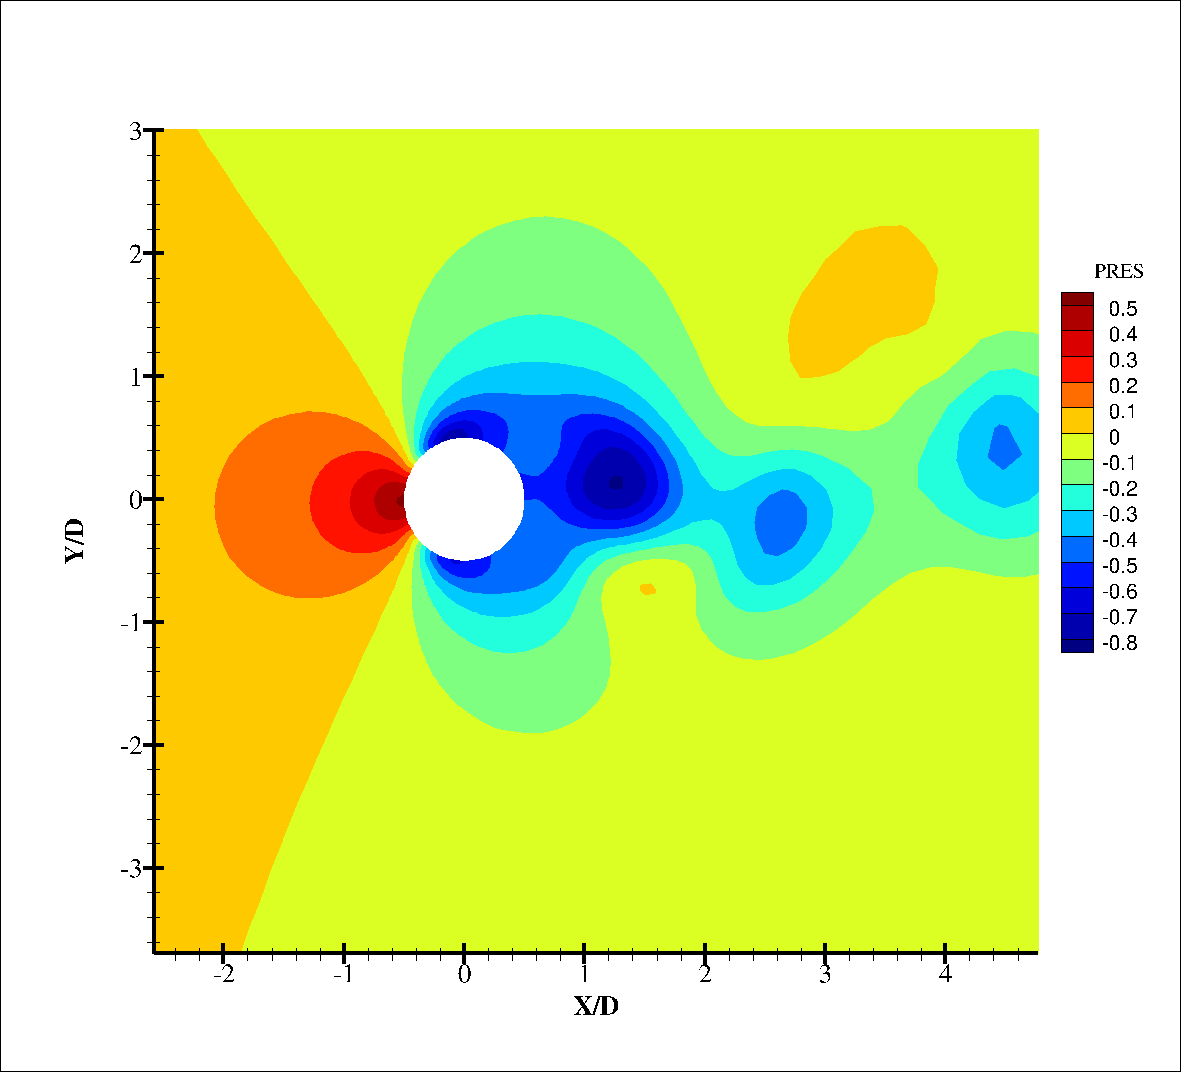
\includegraphics[width=6.5cm]{Pr_cyl_184s}}
		\caption{t=184s}
	\end{subfigure}
	
	\begin{subfigure}[t]{7cm}
		\fbox{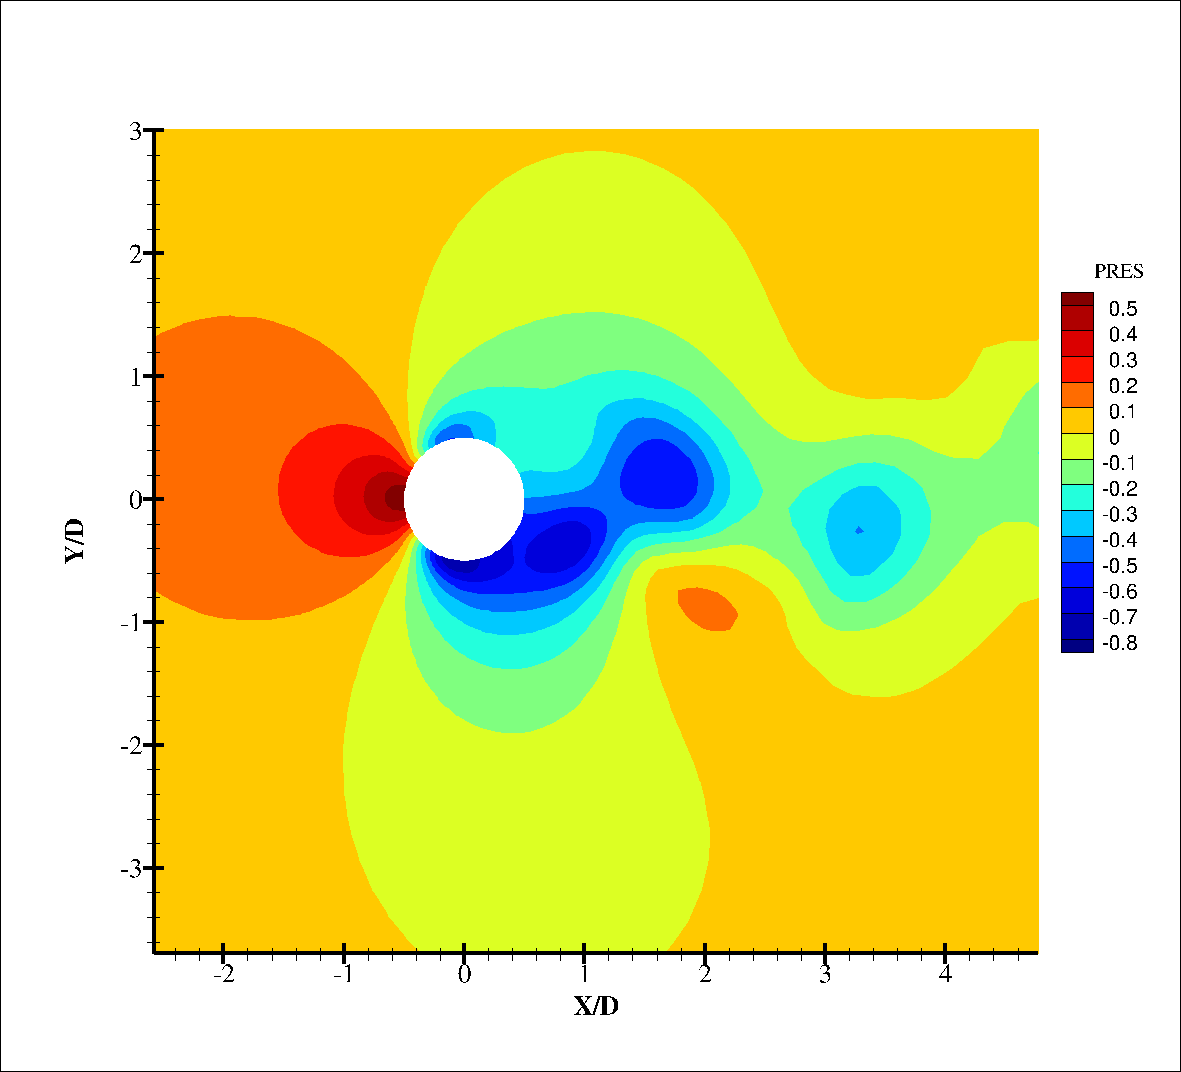
\includegraphics[width=6.5cm]{Pr_cyl_185s}}
		\caption{t=185s}
	\end{subfigure}
%	\hspace{4cm}
	\begin{subfigure}[t]{7cm}
%		\centering
		\fbox{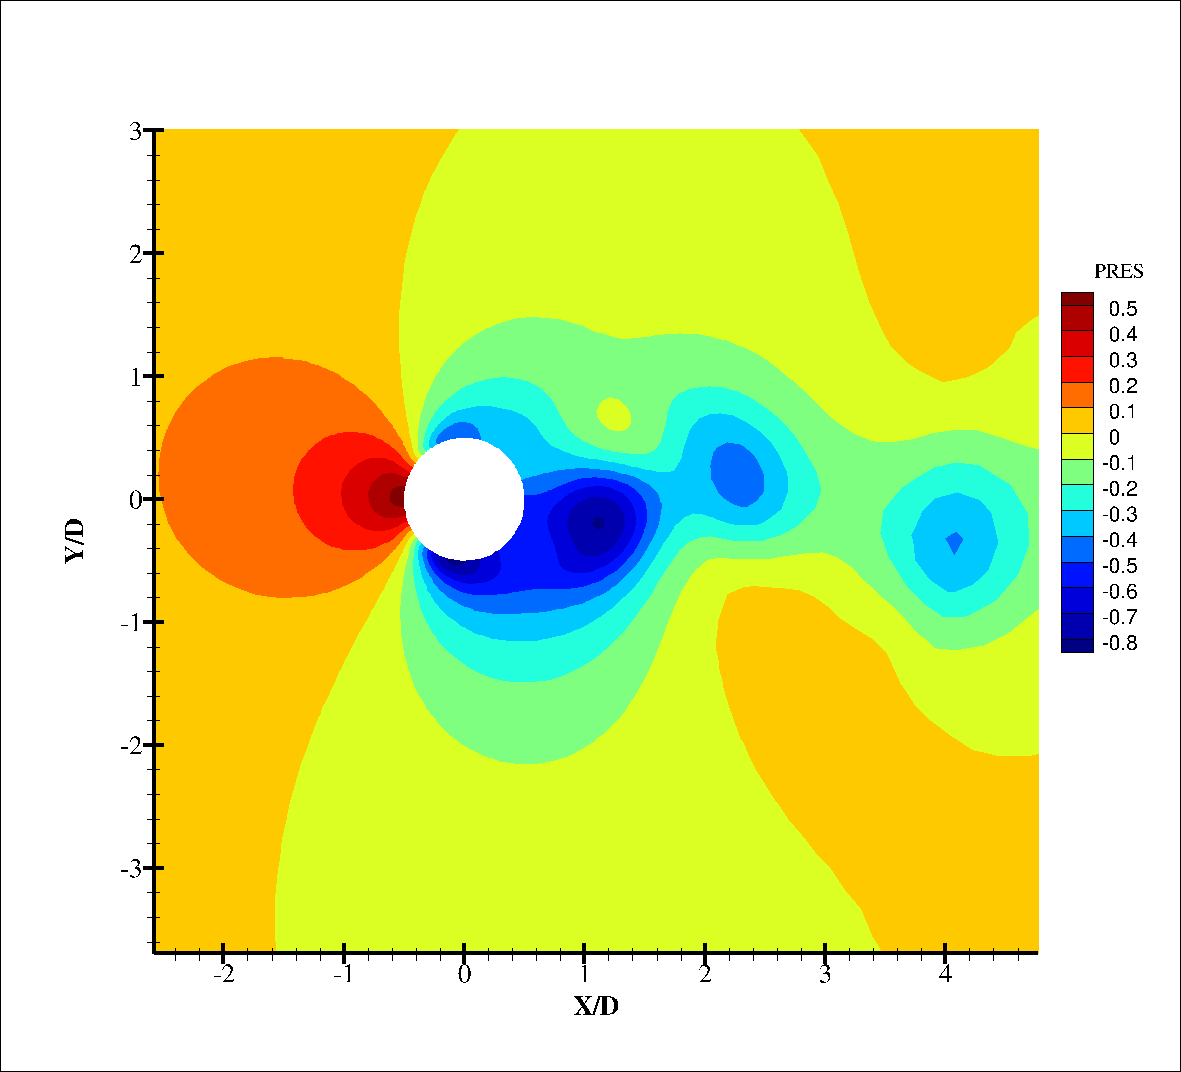
\includegraphics[width=6.5cm]{Pr_cyl_186s}}
		\caption{t=186s}
	\end{subfigure}
\caption{Instantaneous pressure contour}
\label{fig:4.3}
\end{figure}

The \textit{lift} $C_l$ and \textit{drag} $C_d$ coefficients are calculated using the following formulae:

\begin{align}
C_d &= \frac{F_x}{\frac{1}{2} \rho A U_{\infty}^{2}}\\
C_l &= \frac{F_y}{\frac{1}{2} \rho A U_{\infty}^{2}}
\end{align}

In the figure \ref{fig:4.4} the variation of lift and drag coefficients over time is presented. It can be observed that the lift force settles to a sinusoidal pattern after the wake of instability leads to vortex shedding. The root mean square (rms) value of lift coefficient is calculated to be $C_{l_{rms}} = 0.3249$. Similarly, the drag force also follows a periodic behavior with the mean value calculated to be $\bar{C_d} = 1.1632$. 

\begin{figure}[H]
\centering
\fbox{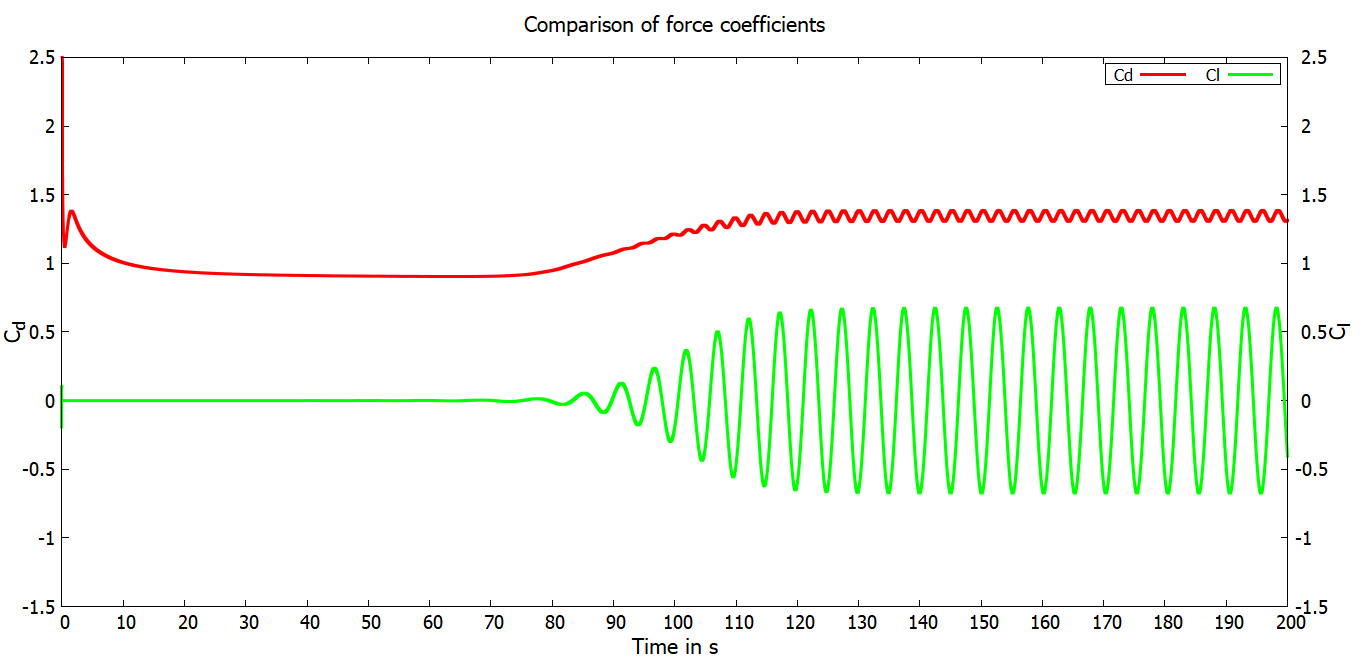
\includegraphics[width=\linewidth]{FC_flow_alone}}
\caption{Variation of Lift and Drag coefficients}
\label{fig:4.4}
\end{figure}

The Strouhal number (St) is a dimensionless number which describes the mechanisms of an oscillating flow. It is defined as,

\begin{equation}
St = \frac{f_s D}{U_\infty}
\end{equation}

where $f_s$ is the vortex shedding frequency. The strouhal number for lift and drag coefficients are calculated to be 0.1945 and 0.3839 respectively. The frequency of oscillation of the drag force is observed to be almost twice as that of lift force. These values are in good agreement to the values observed by \citet{zhou1999vortex}. The observed values are tabulated in \ref{table:4.3}.

\begin{table} [H]
\centering
	\begin{tabular}{|c|c|c|}
	\hline 
	\multirow{2}{*}{Values} & \multicolumn{2}{c|}{Force coefficients}\tabularnewline
	\cline{2-3} 
	 & Coefficient of drag ($C_{d}$) & Coefficient of lift ($C_{l}$)\tabularnewline
	\hline 
	Mean & 1.1632 & -\tabularnewline
	\hline 
	RMS & - & 0.3249\tabularnewline
	\hline 
	Strouhal number (St) & 0.3839 & 0.1945\tabularnewline
	\hline 
	Strouhal number Zhou et.al. (St) & 0.3853 & 0.1922\tabularnewline
	\hline 
	\end{tabular}
\caption{Characteristic values of lift and drag forces}
\label{table:4.3}
\end{table}

This simulation file is used as a restart file for some of the simulation cases of the Fluid-Structure Interaction problem.

\section{FSI simulation results}
The calculations were then performed for an elastic circular cylinder with two degrees of freedom for a number of cases. The values Re=200 and a Mass ratio M=1 is maintained constant through all simulation cases. The damping coefficient Sg is varied for values 1,0.1 and 0.01 respectively and its characteristics are studied. The simulations are carried out for FASTEST-3D with

\begin{enumerate}[(i)]
\item Constant URF (Constant)
\item Aitken URF method (Aitken)
\item Steepest Descent URF method (SD)
\end{enumerate}

The nomenclature given in the brackets for each method is followed in the plots, so as to provide brevity. These cases are simulated with and without a flow restart file, in which the flow field is established. The simulated cases are summarized in the table \ref{table:4.4}.

% Table generated by Excel2LaTeX from sheet 'Sheet1'
\begin{table}[htbp]
  \centering
  \setlength\aboverulesep{0pt}
  \setlength\belowrulesep{0pt} % to avoid discontinuous vertical lines
 \setcellgapes{3pt}\makegapedcells
   \scalebox{0.75}{
    \begin{tabular}{|c|l|c|c|c|c|c|c|}
    \toprule
          & \multicolumn{7}{c|}{M=1} \\
\cmidrule{2-8}          &       & \multicolumn{2}{c|}{Sg=1} & \multicolumn{2}{c|}{Sg=0.1} & \multicolumn{2}{c|}{Sg=0.01} \\
\cmidrule{3-8}          &       & \multicolumn{1}{l|}{With restart} & \multicolumn{1}{l|}{Without restart} & \multicolumn{1}{l|}{With restart} & \multicolumn{1}{l|}{Without restart} & \multicolumn{1}{l|}{With restart} & \multicolumn{1}{l|}{Without restart} \\
    \midrule
    \multirow{3}[6]{*}{FASTEST 3-D with} & Constant URF & x     & x     & x     & x     & x     & x \\
\cmidrule{2-8}          & Aitken URF & x     & x     & x     & x     & x     & x \\
\cmidrule{2-8}          & SD URF & x     & x     & x     & x     & x     & x \\
    \bottomrule
    \end{tabular}%%
   }
  \caption{Summary of the various cases simulated}
  \label{table:4.4}%
\end{table}%

The following nomenclature has been followed henceforth for identifying the different simulation cases:

\begin{enumerate}[(a)]
\item case 1 : Mass ratio M=1 and damping coefficient Sg=1
\item case 2 : Mass ratio M=1 and damping coefficient Sg=0.1
\item case 3 : Mass ratio M=1 and damping coefficient Sg=0.01
\end{enumerate}

\subsection{Determining a suitable constant value of URF}
The simulations were performed considering 50 sub-iterations as the upper limit for convergence of the FSI solver within a time step. To determine a suitable constant value for under-relaxation factor (URF) simulations were carried out for all the cases with different URF values. The simulations were performed on 8 cores for a total of 10,000 time steps. The average sub-iterations taken per time step for various cases is summarized in the table \ref{table:4.5}.\\

\begin{table}[htbp]
  \centering
  	\begin{tabular}{|c|c|c|c|}
	\hline 
	\multirow{2}{*}{FASTEST-3D with constant URF values} & \multicolumn{3}{c|}{Average sub-iterations per timestep}\tabularnewline
	\cline{2-4} 
	 & case 1 & case 2  & case 3\tabularnewline
	\hline 
	0.2 & 32 & 36 & 31\tabularnewline
	\hline 
	0.4 & 14 & 17 & 14\tabularnewline
	\hline 
	0.6 & 15 & 15 & 14\tabularnewline
	\hline 
	\rowcolor[rgb]{ .573,  .816,  .314} 0.8 & 13 & 13 & 11\tabularnewline
	\hline 
	1 & 16 & 16 & 12\tabularnewline
	\hline 
	\end{tabular}
  \caption{Average number of sub iterations per time step}
  \label{table:4.5}%
\end{table}%

The constant URF value of 0.8 gave an average sub-iteration count of around 13 for each of the simulated cases. This value is observed to be an optimum value and the same value has been considered for further simulations.

\subsection{Results for case 1: M=1 and Sg=1}
This section deals with the presentation and discussion of results for the case simulated with Mass ratio M=1 and damping coefficient Sg=1. Each simulation is performed for a total of around 50 vortex shedding cycles and with a frequency ratio $f_n/f_s = 1$. $f_n$ is the natural frequency of the cylinder.

The following nomenclature is followed to represent the characteristic behavior of the system.

\begin{enumerate}[(i)]
\item Mean value of drag coefficient ($\bar{C_d}$)
\item Root Mean Square (RMS) value of lift coefficient ($C_{l,rms}$)
\item Minimum displacement value along flow direction (${X/D}_{min}$)
\item Maximum displacement value along flow direction (${X/D}_{max}$)
\item Minimum displacement value perpendicular to the flow direction (${Y/D}_{min}$)
\item Maximum displacement value perpendicular to the flow direction (${Y/D}_{max}$)
\item Peak-to-peak vibration amplitude ($2 {Y_{rms}}/D$)
\end{enumerate}

All the values are non-dimensionalized in order to have a comparison with the work of \citet{zhou1999vortex}. 

\subsubsection{Without a restart file}
In this simulation, the cylinder is suspended from the initial time. The characteristics of the system is studied. Flow-induced vibrations are in general observed to be non-linear. The vibration of the structure affects the fluid flow around the structure which, in turn, changes the induced forces on the structure and thus the structural response. 

The following nomenclature for the simulation with different under relaxation factor schemes is :

\begin{enumerate}[(a)]
\item FASTEST-3D with constant URF value of 0.8: Constant
\item FASTEST-3D with Aitken URF scheme: Aitken
\item FASTEST-3D with Steepest Descent URF scheme: SD
\end{enumerate} 

In the figure \ref{fig:4.5} the variation of force coefficients $C_d$ and $C_l$ is plotted for a certain period of time steps. It can be observed that the onset of the oscillations are little different for each of the relaxation schemes. This is attributed to the varying number of sub-iterations for each scheme and hence, the convergence. 

\begin{figure}[H]
\centering
\fbox{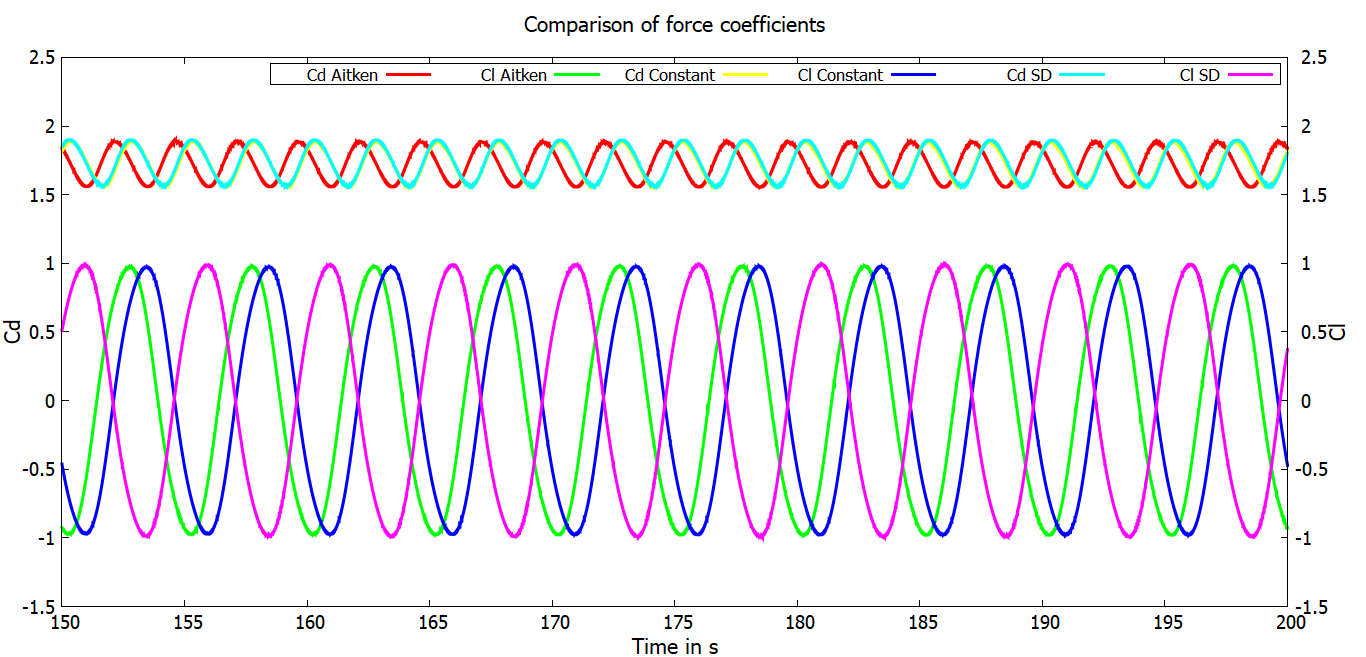
\includegraphics[width=\linewidth]{FC_Sg1_wor}}
\caption{Variation of Drag and Lift coefficients for case 1 without any restart}
\label{fig:4.5}
\end{figure}

The mean value of drag coefficient $\bar{C_d}$ is calculated to be around 1.72 for all the three under relaxation schemes. The rms value of lift coefficient $C_{l,rms}$ is calculated to be around 0.7. These values are in good concordance with the values of \citet{zhou1999vortex}.

In the figure \ref{fig:4.6} the oscillation of the cylinder is quantified and plotted against a certain period of time. As observed in the previous plot, the onset of oscillation for different under relaxation schemes is observed to be varying.

\begin{figure}[H]
\centering
\fbox{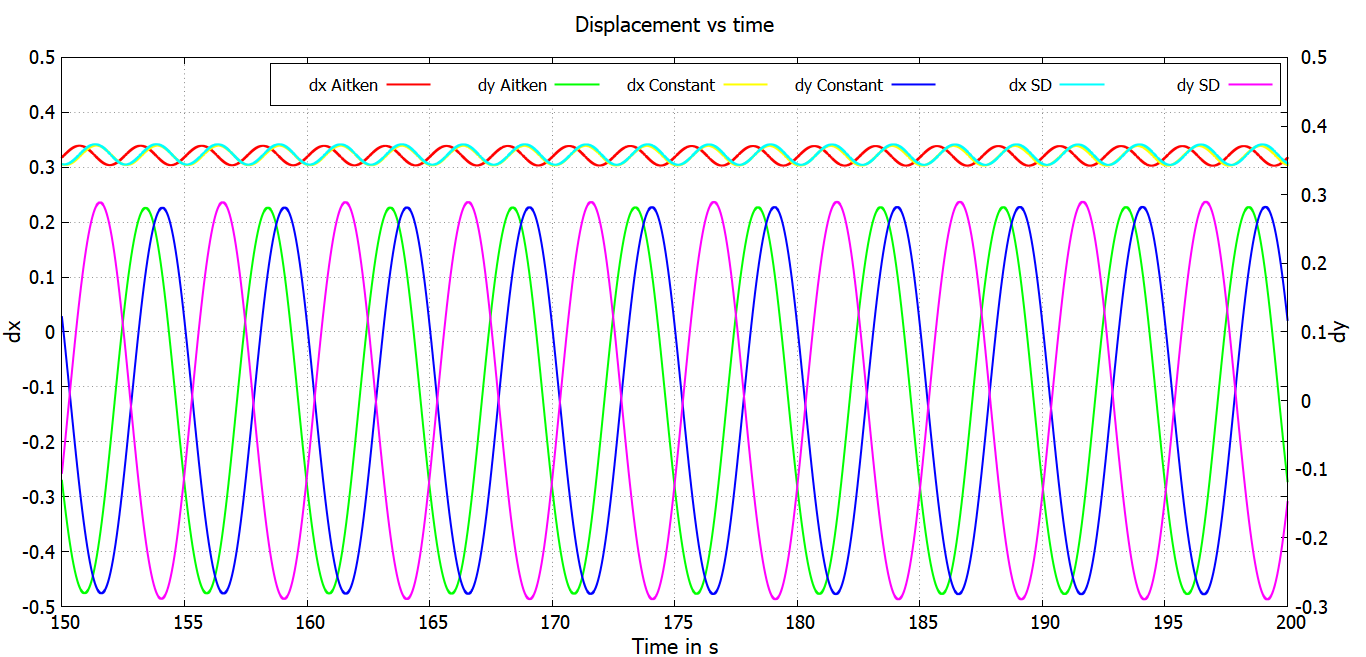
\includegraphics[width=\linewidth]{DC_Sg1_wor}}
\caption{Variation of displacements vs time}
\label{fig:4.6}
\end{figure}
